\documentclass[11pt]{article} % use larger type; default would be 10pt
\usepackage[utf8]{inputenc} % set input encoding (not needed with XeLaTeX)
\usepackage{fullpage}
\usepackage{graphicx} % support the \includegraphics command and options
\usepackage{amsmath}
\usepackage{amssymb}
\newcommand{\drv}[2]{\ensuremath{\frac{d #1}{d #2}}}
\newcommand{\into}{\ensuremath{\int_{-1}^1}}
\newcommand{\intz}{\ensuremath{\int_0^1}}
\newcommand{\intf}{\ensuremath{\int_{-\infty}^\infty}}
\newcommand{\inti}{\ensuremath{\int_{x_{i-1/2}}^{x_{i+1/2}}}}
\newcommand{\intO}{\ensuremath{\int_{4\pi}}}
\newcommand{\order}[1]{\ensuremath{\mathcal{O}(#1)}}
\newcommand{\He}{\ensuremath{\mbox{He}}}
\DeclareMathOperator{\erf}{erf}

\title{Deterministic Uncertainty Quantification with Raven}
\author{\LARGE{Paul Talbot}\\\normalsize{ talbotp@unm.edu}}
%\date{}

\begin{document}
\maketitle

%%%%%%%%%%%%%%%%%%%%%%%%%%%%%%%%%%%%%
\section{Introduction}
RAVEN (Reactor Analysis and Virtual control ENvironment) is a software framework that acts as the control logic driver for thermal hydraulic code RELAP-7.  Central to the purpose of RELAP-7 is determining safety margins in accident-type scenarios for light water nuclear reactors.  

Because the inputs to RELAP-7 are likely to have some level of uncertainty in them, RAVEN allows for the capability to use brute-force Monte Carlo to quantify output uncertainty in terms of input uncertainty.  This makes it valuable as a PRA (probability risk assessment) code, and allows users to more clearly understand margins calculated with RELAP.  

We propose a method of stochastic collocation methods along with generalized polynomial chaos to sample from the uncertainty space of input variables RELAP in an intelligent way and propagate those uncertainties through the code, leveraging RAVEN's interface.  This avoids the need to introduce stochastic noise from Monte Carlo calculations and, for a limited number of uncertain inputs, offers significant speedup over brute force Monte Carlo for the same degree of precision.  Stochastic collocation may be slower than Monte Carlo as the number of uncertain variables grows, but much of this loss can be gained by employing sparse grid methods to reduce the number of necessary samples.  The accuracy cost in stochastic collocation and generalized polynomial chaos originates in truncating infinite sums to a small number of terms; the accuracy of the method generally increases with increasing terms.

We intend eventually to extend the uncertainty quantification tools in RAVEN to propagate uncertainty from inputs of one code through other coupled mutliphysics models in the MOOSE (multiphysics object-oriented simulation environment) system.  Of particular interest is BISON, a fuels performance code, which could in turn provide inputs for RAVEN.
\section{gPC: Generalized Polynomial Chaos}
In general, stochastic processes can be represented efficiently by a basis consisting of an orthogonal set of polynomials, especially if chosen correctly.  While homogeneous chaos only makes use of Hermite polynomials, a more generalized polynomial chaos (gPC) intelligently selects basis polynomials based on weighting functions.
\begin{center}
\begin{tabular}{c c c c}
Polynomial & Random Distr. & Weighting & Span \\ \hline
Legendre & Uniform & 1/2 & [-1,1] \\
Hermite & Normal &  $\exp(-x^2)/\sqrt{2\pi}$ & $(-\infty,\infty)$ \\
Laguerre & Gamma & $x^{k-1}\exp(-x)/\Gamma(k)$ & $[0,\infty)$
\end{tabular}
\end{center}
Consider an uncertain (and therefore treated as stochastic) process $U(p;\zeta)$ that is a function of its ``certain'' input parameters and phase space $p$ as well as uncertain parameters $\zeta$.  In general, $\zeta$ may be the combination of many ($\zeta_1,\zeta_2,...,\zeta_n,...,\zeta_N$) if $U$ depends on many uncertain parameters.  We wish to expand $U$ in terms of one of the polynomial bases in order to quantify its uncertainty.  The polynomial basis is chosen based on the form and span of the uncertainty, as shown in the table.  For any case, $U$ is expanded as
\begin{equation}
U(p;\zeta)\approx\sum_{i=1}^{I} c_i B_i(\zeta),
\end{equation}
where the approximation is because of term truncation at $P_t<\infty$, $c_i$ are polynomial coefficients, and $B_i$ is the polynomial of order $i$ that best fits the uncertainty in $U$.  Since the polynomials are known, we can solve for the unknown coefficients using the orthogonality of the basis polynomials as
\begin{equation}
c_i=\frac{(U(p;\zeta),B_i(\zeta))}{(B_i(\zeta)^2)},
\end{equation}
using $(\cdot)$ as inner product notation
\begin{equation}
\big(f(x),g(x) \big)\equiv \int_S f(x)g(x)dx,
\end{equation}
where $S$ is the support of $x$.


\section{SCM: Stochastic Collocation Method}
The stochastic collocation method (SCM) makes use of quadrature sets to sample from the random space generated by uncertainty.  We can make use of quadrature sets consisting of roots of the same polynomials used as basis functions in order to calculate the inner product for the gPC coefficients,
\begin{align}
(U,B_i)&\equiv\int U(\zeta) B_i(\zeta)d\zeta, \\
  &=\left( \int d\zeta_1 \int d\zeta_2 ... \int d\zeta_N\right)
        U(p;\zeta_1,\zeta_2,...,\zeta_N)B_i(\zeta_1,\zeta_2,...,\zeta_N), \\
 &\approx\left(\sum_{m_1=1}^{M_1}w_{m_1}\sum_{m_2=1}^{M_2}w_{m_2}...\sum_{m_N=1}^{M_N}w_{m_N}\right)
        U(p;\zeta_{m_1},\zeta_{m_2},...,\zeta_{m_N})B_i(\zeta_{m_1},\zeta_{m_2},...,\zeta_{m_N}),
\end{align}
where $w_{m_n}$ are weights obtained from quadrature sets corresponding to the polynomial basis chosen.  The quadrature set may or may not have the same level of truncation as the polynomial expansion; that is, $M_n$ need not be the same as $M_1$ or $I$.

We can further modify the inner product calculation by finding the coefficient term at node $\zeta_m\equiv(\zeta_{1,m_1},...,\zeta_{n,m_n},...,\zeta_{N,m_N})$ so that
\begin{align}
c_i&=\left(\sum_{m_1=1}^{M_1}w_{m_1}\sum_{m_2=1}^{M_2}w_{m_2}...\sum_{m_N=1}^{M_N}w_{m_N}\right)
        c_i(\zeta_{1,m_1},...,\zeta_{n,m_n},...,\zeta_{N,m_N}),\\
  &= \left(\sum_{m_1=1}^{M_1}w_{m_1}\sum_{m_2=1}^{M_2}w_{m_2}...\sum_{m_N=1}^{M_N}w_{m_N}\right)
        c_{i,m},\\
c_{i,m}&\equiv U(p;\zeta_m)B_i(\zeta_m),
\end{align}
where $c_{i,m}$ is the coefficient to the $i$-th order basis polynomial corresponding to a single sample realization $m$ of $U(p;\zeta)$.  Furthermore, we bring weights inward and multiply them to obtain weights that also correspond to a single realization $m$ of $U$, so that
\begin{equation}
w_m=\prod_{h=1}^N w_{m_h},
\end{equation}
\begin{equation}
c_i=\left(\sum_{m_1=1}^{M_1}...\sum_{m_n=1}^{M_n}...\sum_{m_N=1}^{M_N}\right)w_m c_{i,m}.
\end{equation}

\subsection{Constructing Multidimensional Bases}
We now give examples of expanding a multivariate function in multiple bases.  In future sections we explore alternate distributions and polynomials, as well as mapping uncertain spaces onto the [0,1] normalized shifted Legendre polynomial space; for now, we assume all random variables $\zeta_n$ are already expressed as uncertain variables with values $\in[0,1]$.

\subsubsection{Polynomials and Distributions}
We consider a set of eight typical uncertainty distributions and their corresponding polynomials and quadrature.  We summarize them in the table below, taken from TODO CITE Xiu and Karniadakis.  
\begin{center}
\begin{tabular}{c|c|c|c}
 & Unc. Distribution & Basis Polynomials & Support \\ \hline\hline
Continuous & Normal & Hermite & $(-\infty,\infty)$ \\
 & Gamma & Laguerre & $[0,\infty)$ \\
 & Beta & Jacobi & $[a,b]$ \\
 & Uniform & Legendre & $[a,b]$
\end{tabular}
\end{center}
Definitions and examples of these distributions are included in the appendix.
\subsubsection{A Note on Scaling Distributions}
For the distributions described below, integrals are approximated using various Gauss quadratures.  In general, quadrature points for evaluation are easily obtained for standard versions of the distributions; for example, Legendre quadrature evaluates between [-1,1] instead of [$a,b$], and Hermite quadrature evaluates on a distribution with 0 mean and 1 variance instead of $\mu$ mean and $\sigma^2$ variance.  As such, it is practical to scale a distribution with a substitution of variables in order to obtain the standard distribution.  We provide rules for this scaling for each distribution.  Special care must be made when changing variables in the coefficient integrations, however, to include the Jacobian and change of limits where applicable.  The appropriate adjustments are made in the examples below.  

The procedures exemplified here start by scaling to the standardized distribution $\zeta$ from the actual distribution $\xi$.  A general rule will be given of the form $\zeta(\xi)$ before performing the analysis to obtain the expansion for $\hat f(\zeta)$.  In order to obtain values using inputs in the distribution of $\xi$, it is only necessary to first make the conversion $\xi(\zeta)$.  For instance, if a uniform uncertainty variable ranges from $a$ to $b$, the conversion rule is
\begin{equation}
\zeta(\xi)=\frac{b-a}{2}\xi+\frac{a+b}{2},\hspace{20pt}\zeta\in[0,1],
\end{equation}
and, once $\hat f(\zeta)$ is obtained, evaluating $f(\xi)$ is performed by
\begin{equation}
f(\xi)=f(\xi(\zeta))=\hat f\left(\frac{2}{b-a}\left[\xi-\frac{a+b}{2}\right]\right).
\end{equation}

\subsubsection{Example: Single-Dimensional Legendre expansion}
Starting with the simplest case, we consider a function of a single uniform-uncertainty variable $\zeta$,
\begin{equation}
f(\xi)=a+b\xi, \hspace{10pt}\xi\in[a,b],
\end{equation}
where $a,b$ are scaling constants.  We can in general scale this function to $a=0,b=1$ using the rule
\begin{equation}
\zeta=\frac{b-a}{2}\xi+\frac{a+b}{2},\hspace{20pt}\zeta\in[0,1].
\end{equation}
We expand $f(\zeta)$ in normalized shifted Legendre polynomials,
\begin{align}
f(\zeta)&=\sum_{i=0}^\infty f_i\tilde P_i(\zeta),\\
 &= \sum_{i=0}^1 f_i\tilde P_i(\zeta).
\end{align}
We can truncate the sum at 1 term because we know a priori $f(\zeta)$ is order 1 in $\zeta$, so it can be exactly represented by Legendre polynomials of up to order 1; in general, this is not known and perfect accuracy can only be guaranteed with infinite terms.  Using the orthogonality of the normalized shifted Legendre polynomials, we find the coefficients $f_i$ given by
\begin{equation}
f_i=\intz f(\zeta)\tilde P_i(\zeta)d\zeta.
\end{equation}
We can approximate the integral with shifted Gauss-Legendre quadrature,
\begin{align}
f_i&=\sum_{\ell=0}^\infty w_\ell f(\zeta_\ell)\tilde P_i(\zeta_\ell),\\
 &=\sum_{\ell=0}^1 w_\ell f(\zeta_\ell)\tilde P_i(\zeta_\ell),
\end{align}
where once again, because we know the shifted Legendre polynomial order is no greater than 1 and $f(\zeta)$ is order 1, the integral has maximum order 3 and shifted Legendre quadrature can exactly integrate polynomials of order $2n-1$.  It is straightforward to insert the values from the shifted Legendre quadrature set and see that the coefficients obtained are
\begin{equation}
f_0=a+\frac{b}{2},\hspace{10pt} f_1=\frac{b\sqrt{3}}{6},\hspace{10pt} f_{i>1}=0.
\end{equation}
If we reconstruct $f(\zeta)$ using these coefficients and the first three normalized Legendre polynomials, we obtain our original function $a+b\zeta$.

%\subsubsection{Example: Single-Dimensional Hermite expansion}
%We now consider a function of a single normal-uncertainty variable $\xi$,
%\begin{equation}
%f(\xi)=\frac{1}{\sqrt{2\pi b}}\exp\left(-\frac{(\xi-a)^2}{2b}\right),\hspace{20pt}\zeta\in(-\infty,\infty),
%\end{equation}
%where $a,b$ are scaling constants.  We can in general scale this function to $a=0,b=1$ using the rule
%\begin{equation}
%\xi=b\zeta+a,
%\end{equation}
%\begin{equation}
%f(\zeta)=\frac{1}{\sqrt{2\pi b}}\exp\left(-\frac{\zeta^2}{2}\right).
%\end{equation}
%We expand similar to the Legendre case but with normalized probabilist Hermite polynomials $\He_n$,
%\begin{equation}
%f(\zeta)=\sum_{i=0}^\infty f_i \He_i(\zeta)W_H(\zeta).
%\end{equation}
%We note here the inclusion of the weighting function $W_H $.  This function is the probability distribution of f(x).  For Gaussian-distributed uncertainty, this is given as
%\begin{equation}
%W_H(\zeta)=e^{-\frac{x^2}{2}}.
%\end{equation}
%In the Legendre case, the weighting function is unity and $W$ was omitted.
%Using orthogonality,
%\begin{equation}
%f_i=\intf f(\zeta)\He_i(\zeta)d\zeta.
%\end{equation}
%To integrate this integral using Hermite quadrature, we first recognize
%\begin{equation}
%\intf f(x)e^{-x^2/2}dx=\intf f(x)W_H(x)=\sum_{\ell=0}^\infty w_\ell f(x_\ell),
%\end{equation}
%\begin{equation}
%\intf f(x)dx=\intf \frac{f(x)}{W_H(x)}W_H(x)dx=\sum_{\ell=0}^\infty w_\ell \frac{f(x_\ell)}{W_H(\ell)}.
%\end{equation}
%We demonstrate the utility of this procedure by example, expanding $f(\zeta)/W_H(\zeta)$,
%\begin{align}
%\intf f(\zeta)dx&=\intf \frac{f(\zeta)}{W_H(\zeta)}W_H(\zeta)d\zeta,\\
%&=\intf \frac{\frac{1}{\sqrt{2\pi b}}\exp\left(-\frac{\zeta^2}{2}\right)}{e^{-\frac{\zeta^2}{2}}}W_H(\zeta)d\zeta,\\
%&=\intf \frac{1}{\sqrt{2\pi b}} W_H(\zeta)d\zeta,\\
%&=\frac{1}{\sqrt{2\pi b}}\sum_{\ell=0}^\infty w_\ell.
%\end{align}
%%The utility of the quadrature choice lies in the fact that $f(x)$ and $W_H(x)$ are similar in form, resulting in simplification.  Thus, our coefficient integral becomes
%Even if $f(\zeta)$ is not identical to $W_H(\zeta)$, it is useful for them to have the same form.  Returning to our coefficient integral,
%\begin{align}
%f_i&=\intf f(\zeta)\He_i(\zeta) d\zeta,\\
%  &=\intf \frac{f(\zeta)\He_i(\zeta)}{W_H(\zeta)}W_H(\zeta)d\zeta,\\
%  &=\sum_{\ell=0}^\infty w_\ell\frac{f(\zeta_\ell)\He_i(\zeta_\ell)}{W_H(\zeta_ell)}.
%\end{align}

\subsubsection{Example: Multivariate Expansion}
We now consider multidimensional function of $\zeta_1,\zeta_2$,
\begin{equation}
f(\zeta)\equiv f(\zeta_1,\zeta_2)=(a-b\zeta_1)(c-d\zeta_2),
\end{equation}
where $(a,b,c,d)$ are arbitrary scalars.  We expand each dimension in normalized shifted Legendre polynomials,
\begin{equation}
f(\zeta)=\sum_{i_1=0}^\infty \sum_{i_2=0}^\infty f_{i_1,i_2}\tilde P_{i_1}(\zeta_1)\tilde P_{i_2}(\zeta_2),
\end{equation}
where $f_{i_1,i_2}$ is the combined coefficient for the multivariate polynomial term.  The coefficients can be obtained in the same manner as the single dimension expansion,
\begin{equation}
f_{i_1,i_2}=\intz\intz f(\zeta)\tilde P_{i_1}(\zeta_1)\tilde P_{i_2}(\zeta_2)d\zeta_1d\zeta_2,
\end{equation}
and approximated with Legendre quadrature
\begin{align}
f_{i_1,i_2}&=\sum_{\ell_1=0}^\infty w_{\ell_1} \sum_{\ell_2=0}^\infty w_{\ell_2}
     f(\zeta_{1,\ell_1},\zeta_{1,\ell_2})\tilde P_{i_1}(\zeta_{1,\ell_1})\tilde P_{i_2}(\zeta_{2,\ell_2}),\\
  &=\sum_{\ell_1=0}^\infty \sum_{\ell_2=0}^\infty w_{\ell_1}w_{\ell_2}
     f(\zeta_{1,\ell_1},\zeta_{1,\ell_2})\tilde P_{i_1}(\zeta_{1,\ell_1})\tilde P_{i_2}(\zeta_{2,\ell_2}).
\end{align}
Using the first two terms from each sum, we obtain the coefficients
\begin{align}
f_{0,0}&=\frac{(2a+b)(2c+d)}{4},\\
f_{0,1}&= \frac{d\sqrt{3}}{12}(2a+b), \\
f_{1,0}&=\frac{b\sqrt{3}}{12}(2c+d) \\
f_{1,1}&=\frac{bd}{12},
\end{align}
\begin{align}
f(x,y)&=f_{0,0}\tilde P_0(\zeta_1)\tilde P_0(\zeta_2) +
f_{0,1}\tilde P_0(\zeta_1)\tilde P_1(\zeta_2) +
f_{1,0}\tilde P_1(\zeta_1)\tilde P_0(\zeta_2) +
f_{1,1}\tilde P_1(\zeta_1)\tilde P_1(\zeta_2),\\
&=(a+b\zeta_1)(c+d\zeta_2).
\end{align}

\subsubsection{General Multivariate Expansion}
From the two examples above, it is straightforward to extrapolate the general formulation for an expansion in an unknown number of dimensions.  We consider a function of $\zeta\equiv(\zeta_1,\zeta_2,\cdots,\zeta_n,\cdots, \zeta_N)$
\begin{equation}
f(\zeta)\equiv f(\zeta_1,\cdots,\zeta_n,\cdots, \zeta_N).
\end{equation}
We expand it in $N$ dimensions in normalized shifted Legendre polynomials,
\begin{align}
f(\zeta)&=\sum_{i_1}^\infty \sum_{i_2}^\infty \cdots\sum_{i_N}^\infty 
        f_{i_1,i_2,\cdots,i_N} \prod_{n=1}^N \tilde P_{i_n}(\zeta_n),\\
 &=\sum_{i_1}^\infty \cdots\sum_{i_N}^\infty
        f_{i} \prod_{n=1}^N \tilde P_{i_n}(\zeta_n),
\end{align}
where for simplicity we have defined $f_i$ as the coefficient for the full set of polynomials at a particular set in the sum $i=(i_1,\cdots,i_N)$.  As before, the coefficients $f_i$ are determined using orthogonality,
\begin{equation}
f_i=\into \cdots \into \left[f(\zeta)\prod_{n=1}^N \tilde P_{i_n}(\zeta_n)\right] d\zeta_1\cdots d\zeta_N,
\end{equation}
which is approximated with Legendre quadrature as
\begin{align}
f_i&=\sum_{\ell_1=0}^\infty\cdots\sum_{\ell_N=0}^\infty \left(\prod_{n=1}^N w_{\ell_n}\right) 
              f(\zeta_\ell)\prod_{n=1}^N \tilde P_{i_n}(\zeta_{n,\ell_n}),\\
  &=\sum_{\ell_1=0}^\infty\cdots\sum_{\ell_N=0}^\infty \left(\prod_{n=1}^N w_{\ell_n}\tilde P_{i_n}(\zeta_{n,\ell_n})\right) 
              f(\zeta_\ell), 
\end{align}
where for convenience we define
\begin{equation}
f(\zeta_\ell)\equiv f(\zeta_{1,\ell_1},\cdots,\zeta_{n,\ell_n},\cdots\zeta_{N,\ell_N}).
\end{equation}
In practice, it is computationally effective to store a tensor of coefficients $f_i$ for each abscissa of each quadrature.  This coefficient tensor has dimensionality equal to the number of uncertain parameters $N$, and each dimension has length equal to the number of quadrature abscissa used for that uncertain parameter.  In this case, for a three-variable function, \texttt{coeff[i,j,k]} corresponds to $f_{i,j,k}$.

\subsubsection{Results}
To show the successful expansion of various functions in their corresponding polynomials, we use the method of manufactured solutions to check basic single-output functions against their expansion in polynomial bases.  We use the manufactured solutions
\begin{align}
f(x)&=2x^2+2x+1,\\
f(x,y)&=(1-x)(1-y),\\
f(w,x,y,z)&=wx^2(1-y)(1-z^2).
\end{align}
Graphical representations of the 1D and 2D cases are shown in Figs. \ref{1Derr} and \ref{2Derr}.  In the 1D, 2D, and 4D cases, the l2norm of the error between manufactured and computed solution was less than $1\times10^{-14}$.
\begin{figure}[h!]
\centering
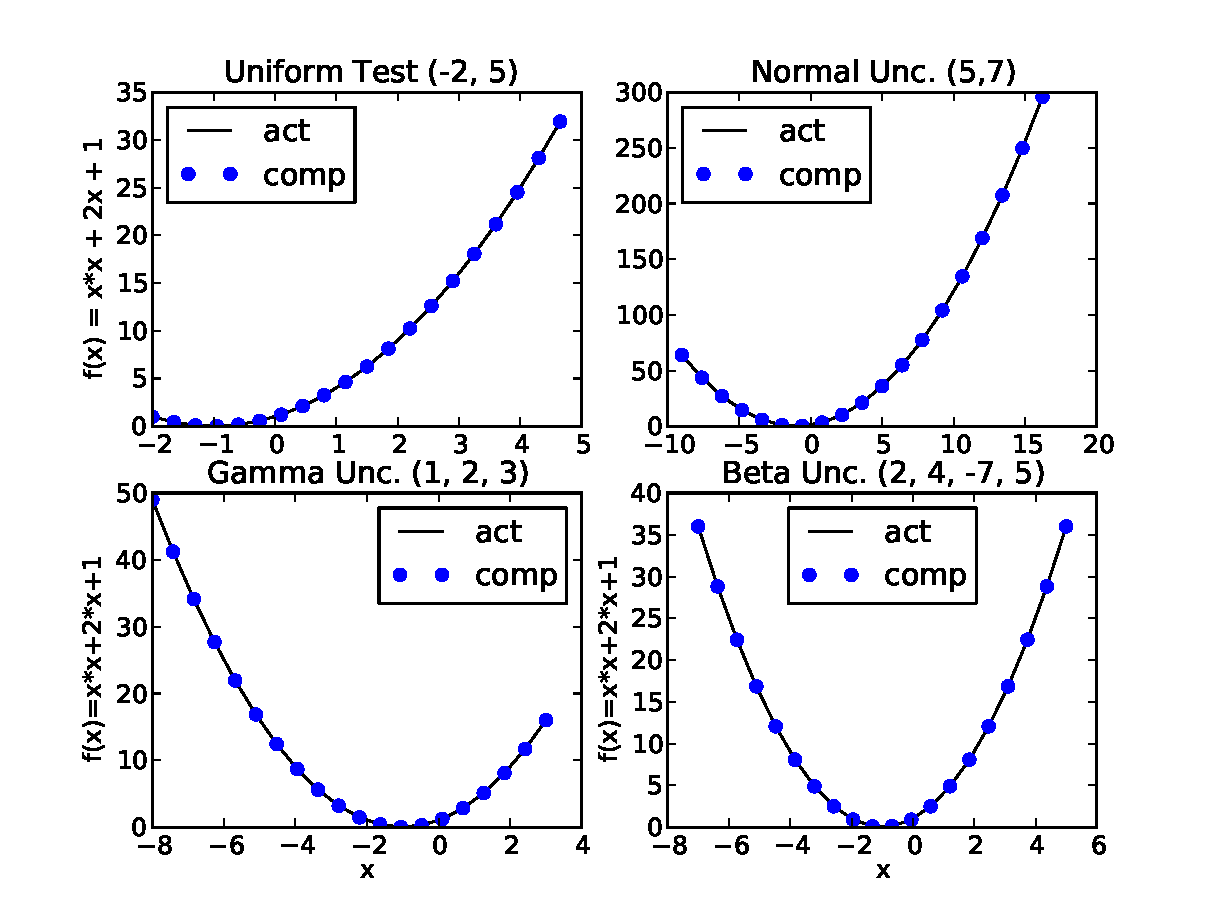
\includegraphics[width=0.7\linewidth]{./graphics/contDistErr}
\caption{1D Examples}
\label{1Derr}
\end{figure}

\begin{figure}[h!]
\centering
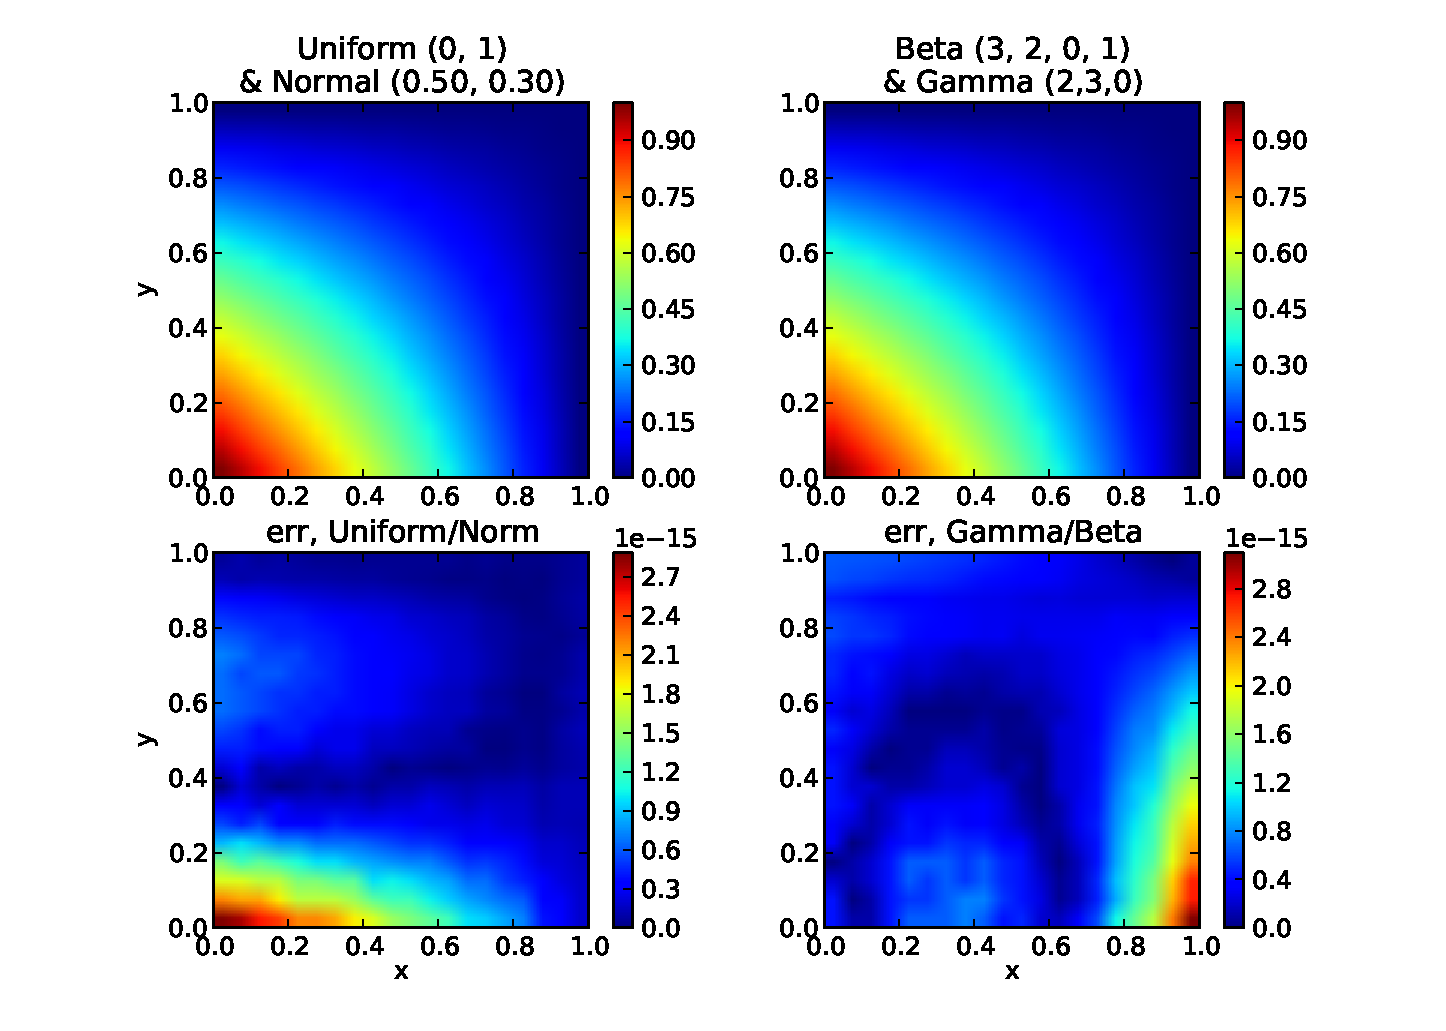
\includegraphics[width=0.7\linewidth]{./graphics/contDistErr2D}
\caption{2D Examples}
\label{2Derr}
\end{figure}

\subsection{Alternative Uncertainties}


\subsubsection{Arbitrary Uncertainties}
While the probability distributions and polynomial chaos above are useful in describing uncertainties, there exist many other possible uncertainty distributions.  However, it is possible to project arbitrary uncertainties into uniform [0,1] space and treat them with shifted Legendre polynomials.  In fact, we require only the percent point (or percentile) distribution of an uncertain variable to create a mapping between its natural domain and the [0,1] domain.  The drawback to this method is that shifted Legendre polynomials may not efficiently describe the distribution, and many terms may be necessary to develop an accurate representation.

We follow here the pattern outlined by TODO CITE Xiu and Kerniadakis. Consider an uncertain parameter $\xi$ with arbitrary probability distribution function $f(\xi)$.  We can expand this parameter in basis polynomials that describe the desired [0,1] space; namely, (normalized) shifted Legendre polynomials $\tilde P_i$,
\begin{equation}
\xi=\sum_{i=0}^\infty \xi_i \tilde P_i.
\end{equation}
As before, we find the coefficients using the orthogonality of, and the inner product in the Hilbert space spanned by, the polynomial basis,
\begin{equation}\label{eqn:nonsense}
\xi_i=\int_S \xi P_i(\zeta)g(\zeta)d\zeta,
\end{equation}
where $g(\zeta)$ is the uniform probability distribution of $\zeta\in [0,1]$. 
We note that Eq. \eqref{eqn:nonsense} is mathematically nonsensical, in that we assume $\zeta$ to be dependent on $\xi$ and their supports are not guaranteed to be the same; that is, they are likely to belong to different probability spaces - if not, then there is no need to perform the mapping.  To correlate the two, we introduce a new uncertain variable $u\in [0,1]$.  Recalling the probability distribution functions $f(\xi)$ and $g(\zeta)$, we transform probability space to show
\begin{equation}
du=f(\xi)d\xi=dF(\xi),\hspace{20pt}du=g(\zeta)=dG(\zeta),
\end{equation}
where $F,G$ are the cumulative distribution function (cdf)'s for $f,g$,
\begin{equation}
F(\xi)=\int_{-\infty}^{\xi}f(s)ds,\hspace{20pt}G(\zeta)=\int_{-\infty}^{\zeta}g(s)ds.
\end{equation}
We require both $\xi$ and $\zeta$ to be mapped to the domain of $u$, and show
\begin{equation}
\xi=F^{-1}(u),\hspace{20pt}\zeta=G^{-1}(u),
\end{equation}
where $F^{-1},G^{-1}$ are the inverse of the cdf, or percent point function (ppf).  Using these transformations, we return to the expansion of $\xi$ and write
\begin{equation}
\xi=\sum_{i=0}^\infty \xi_i P_i,
\end{equation}
\begin{align}
\xi_i&=\intz F^{-1}(u)P_i\big(G^{-1}(u)\big)du,\\
  &=\sum_{n=0}^\infty w_n F^{-1}(u_n)P_i\big(G^{-1}(u_n)\big),
\end{align}
where we have applied shifted Gauss-Legendre quadrature to evaluate the integral.  We note that the only requirement for mapping any arbitrary uncertainty onto a common space is the ability to evaluate the ppf of an uncertainty distribution at quadrature points ($u_n$).  Also, this procedure is general for any pdf $g(\zeta)$ to map $\xi$ onto the domain of $\zeta$; for our purposes, $\zeta\in[0,1]$ is the most beneficial.



%\subsubsection{Uniform Uncertainty with Arbitrary Domain}
%We return to our one-dimensional case to consider any function $f(\xi)$, but allow variable $\xi$ to range on arbitrary [a,b] instead of [-1,1].  We can perform a transformation of variables to project the necessary integrals onto  [-1,1] domain.  We still expand
%\begin{equation}
%f(\xi)=\sum_{i=0}^\infty f_iP_i(\xi),  \hspace{10pt}\xi\in [a,b].
%\end{equation}
%The coefficients $f_i$ are calculated like above, but over the support space [a,b],
%\begin{equation}
%f_i=\int_a^b f(\xi)P_i(\xi)d\xi.
%\end{equation}
%In general, we seek to change variables to enable the transformation
%\begin{equation}
%\int_a^b g(x)dx = \int_{-1}^1k f(y)dy = \sum_{\ell=1}^\infty w_{\ell}kf(y_{\ell}),
%\end{equation}
%where $k$, $y$, and $f(y)$ are unknown and $w_\ell$ are weights from Gauss-Legendre quadrature.
%\begin{equation}\label{eqn:toQuad}
%\into f(y) dy =\sum_{\ell=1}^\infty w_\ell f(y_\ell). %= \int_a^b k g(x)dx.
%\end{equation}
%Because this transformation is linear (changing average and range of the uniform distribution, not the distribution itself) we define
%\begin{equation}
%x=\alpha + \beta y \to y\equiv \frac{x-\alpha}{\beta},
%\end{equation}
%\begin{equation}
%dy = \frac{1}{\beta} dx,
%\end{equation}
%\begin{equation}
%\alpha+\beta a=-1,\hspace{10pt} \alpha+\beta b=1.
%\end{equation}
%This two-variable linear system allows us to solve
%\begin{align}
%\alpha&=\frac{a+b}{2}\equiv \mu,\\
%\beta&=\frac{b-a}{2}\equiv \sigma,
%\end{align}
%where we take the mean $\mu$ and range $\sigma$ from $\xi=\mu\pm\sigma$.  We perform the transformation,
%\begin{equation}
%\into g(y)dy = \beta\int_a^b f\left(\frac{x-\alpha}{\beta}\right)dx=
%      \sigma\int_a^b f\left(\frac{x-\mu}{\sigma}\right)dx =\sigma\int_a^b g(x)dx.
%\end{equation}
%Using Eq. \eqref{eqn:toQuad}, we substitute
%\begin{align}
%\sigma\int_a^b g(x)dx &= \sum_{\ell=1}^\infty w_\ell f(y_\ell),\\
%\int_a^b g(x)dx &= \sum_{\ell=1}^\infty \frac{w_\ell}{\sigma} f(y_\ell),\\
%  &=\sum_{\ell=1}^\infty \frac{w_\ell}{\sigma} f\left(\frac{x_\ell-\mu}{\sigma}\right),\\
%  &=\sum_{\ell=1}^\infty \frac{w_\ell}{\sigma} g(x_\ell).
%\end{align}
%Our effective weights $w'_\ell$ and abscissa $x_\ell$ are modified from original Gauss-Legendre abscissa $y_\ell$ and weights $w_\ell$ by
%\begin{align}
%x_\ell &= \mu+\sigma y_\ell,\\
%w'_\ell &= \frac{w_\ell}{\sigma}.
%\end{align}
%Returning to our coefficient integrals, then,
%\begin{align}
%f_i&=\int_a^b f(\xi)P_i(\xi)d\xi,\\
%  &=\sum_{\ell=1}^\infty \frac{w_\ell}{\sigma} f(\mu+\sigma\xi_{\ell})P_i(\mu+\sigma\xi_\ell).
%\end{align}
%This adjustment allows any uniformly-distributed value to be represented on [-1,1].  We caution that when obtaining values for $f(\xi)$ using the expansion,
%\begin{equation}
%f(\xi)=\sigma f(\zeta),\hspace{20pt}\xi\in[a,b],\zeta\in[-1,1].
%\end{equation}
%
%\subsubsection{Normal Uncertainty on Standard Domain}
%We consider the same function $f(\zeta)$, but change the uncertainty in $\zeta$ to follow a Gaussian (normal) distribution with mean $\mu=0$ and variance $\sigma^2=1$.  The probability distribution function for $\zeta$ is given by
%\begin{equation}
%\zeta(\theta)=\frac{1}{\sqrt{2\pi}} e^{\theta^2/2}.
%\end{equation}
%We also note that $\zeta\in[-\infty,\infty]$.  The [$-\infty,\infty$] domain together with Gaussian distribution make probabilist's (or statistician's, or normalized) Hermite polynomials $\He_n(x)$ more desirable than Legendre polynomials for accuracy with few terms.  Thus, for a monovariate function of a Gaussian-uncertainty parameter,
%\begin{align}
%f(\zeta)&=\sum_{i=0}^\infty f_i \He_i(\zeta),\\
%f_i&=\intf f(\zeta)\He_i(\zeta),\\
%  &=\sum_{h=1}^\infty \frac{w_h f(\zeta_h) \He_i(\zeta_h)}{W_i(\zeta_h)},
%\end{align}
%where $w_h,\zeta_h$ are the weights and abscissa from Gauss-Hermite quadrature, and we introduce $W(\zeta)$ as the weight function corresponding to statistician's Hermite polynomials,
%\begin{equation}
%W_i(\zeta)=\frac{1}{\sqrt{(2\pi)^i}}e^{-\zeta/2}.
%\end{equation}
%A corresponding weighting function exists for the Legendre polynomials, but its value is always unity, and it was omitted from the calculation.

\appendix
\section{Polynomials and Distributions}
For reference we include the polynomial, distribution, and quadrature definitions for the continuous distributions used in this document.  To describe polynomials, we make use of the Pachhammer symbol $(a)_n$
\begin{equation}
(a)_n=a(a+1)(a+2)...(a+n-1),\hspace{10pt}n=1,2,3,...
\end{equation}
with $(a)_n=1$.  The generalized hypergeometric series $_rF_s$ is given by
\begin{equation}
_rF_s(a_1,...,a_r;b_1,...,b_s;z)=\sum_{k=0}^\infty \frac{(a_1)_k\cdots(a_r)_k}{(b_1)_k\cdots(b_s)_k}\frac{z^k}{k!}.
\end{equation}
\begin{figure}[h!]
\centering
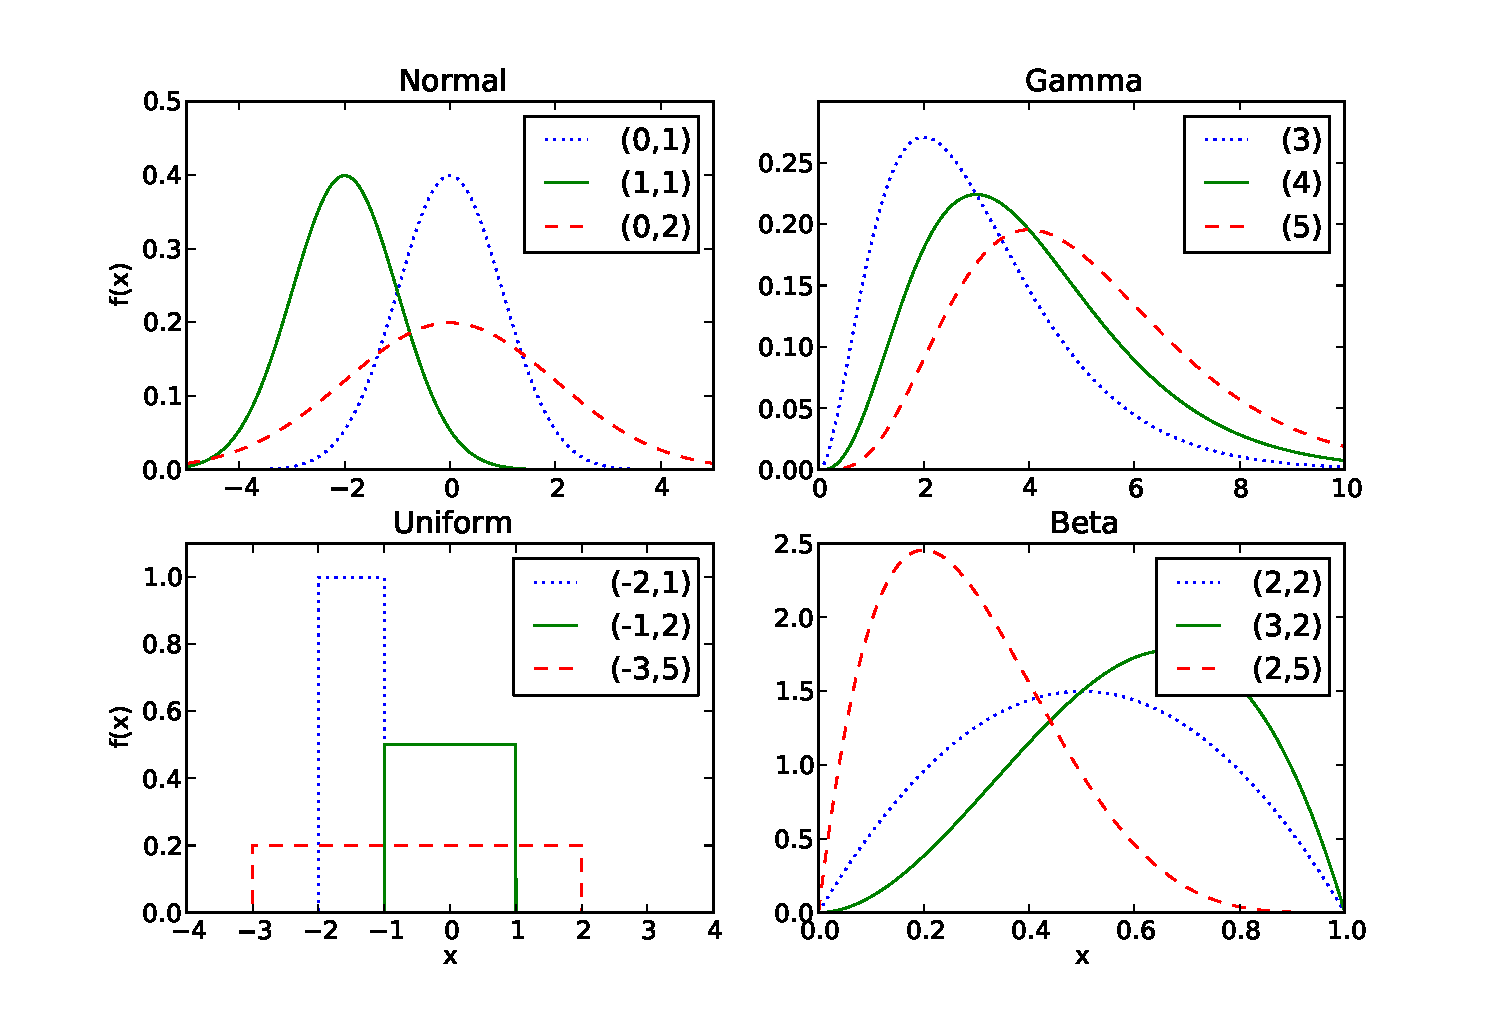
\includegraphics[width=\linewidth]{./graphics/distros}
\caption{Several Distributions}
\label{fig:distros}
\end{figure}

\subsection{Standard Distributions}
There are several standard distributions for which quadratures with corresponding polynomials are well-known, making them efficiently represented with small quadratures.  We present four here: normal, Gamma, uniform, and Beta.

\newpage
\subsubsection{Normal and Hermite $\He_n$}
The normal or Gaussian distribution has support from $-\infty$ to $\infty$ and is characterized by Hermite polynomials, with the associated Gauss-Hermite quadrature.  The pdf of the normal distribution has the form
\begin{equation}
\xi(x;\mu,\sigma^2)=\frac{1}{\sqrt{2\pi\sigma^2}}\exp\left(-\frac{(x-\mu)^2}{2\sigma^2}\right),
      \hspace{10pt} x\in(-\infty,\infty),
\end{equation}
where $\mu,\sigma^2$ are the mean and variance respectively.  Two different kinds of Hermite polynomials exist: one the ``probabilist" Hermite polynomial $\He_n(x)$, and the more often seen ``physicist'' Hermite polynomial $H_n(x)$.  The two are essentially the same with the important exception $H_n(x/\sqrt{2})=\He_n(x)$.
\begin{align}
\He_n&=(-1)^n e^{x^2/2}\frac{d^n}{dx^n}e^{-x^2/2},\\
H_n&=(-1)^n e^{x^2}\frac{d^n}{dx^n}e^{-x^2}.
\end{align}
We make use of the probabilist here because of its conformity with the Gaussian distribution.  The Hermites are orthogonal,
\begin{equation}
\intf \He_m(x)\He_n(x) e^{-x^2/2}dx=\sqrt{2\pi} n! \delta_{nm}.
\end{equation}
Hermite quadrature integrates exactly functions of the kind
\begin{equation}
\intf f(x)e^{-x^2/2}dx=\sum_{\ell=0}^L w_\ell f(x_\ell).
\end{equation}
The abscissas of the quadrature are given by roots of the $\He_n$ polynomial and weights are given by
\begin{equation}
w_\ell = \frac{L!\sqrt{2\pi}}{n^2[\He_{n-1}(x_\ell)]^2}.
\end{equation}
A normal distribution is shown with $\mu=0,\sigma^2=1$ in Fig. \ref{fig:distros}.

\newpage
\subsubsection{Gamma and Laguerre $L_n^\alpha$}
The Gamma distribution has support from 0 to $\infty$ and is characterized by Laguerre polynomials with the associated Gauss-Laguerre quadrature.  The pdf of the Gamma distribution has the form
\begin{equation}
\xi(x;\alpha,\beta)=\frac{x^\alpha e^{-x/\beta}}{\beta^{\alpha+1}\Gamma(\alpha+1)},
    \hspace{10pt}\alpha>-1,\beta>0,x\in(0,\infty),
\end{equation}
\begin{equation}
\Gamma(\alpha)\equiv\int_0^\infty t^\alpha e^{-t}\frac{dt}{t},
\end{equation}
\begin{equation}
\Gamma(\alpha+1)=\alpha\Gamma(\alpha),
\end{equation}
where $\alpha,\beta$ are shape and scale constants, respectively.  The (generalized) Laguerre polynomials $L^{(\alpha)}_n$ are the solutions to the second order PDE
\begin{equation}
xy''+(\alpha+1-x)y'+ny=0,
\end{equation}
and are given by
\begin{align}
L^{(\alpha)}_n(x)&=\frac{x^{-\alpha}e^x}{n!}\frac{d^n}{dx^n}\left(e^{-x}x^{n+\alpha}\right),\\
  &=\frac{(\alpha+1)_n}{n!} {}_1F_1(-n;\alpha+1;x),
\end{align}
\begin{equation}
\int_0^\infty e^x x^\alpha L^{(\alpha)}_m(x) L^{(\alpha)}_n(x)dx=\frac{\Gamma(n+\alpha+1)}{n!}\delta_{mn},
     \hspace{10pt}\alpha>-1.
\end{equation}
General Laguerre quadrature exactly integrates functions of the kind
\begin{equation}
\int_0^\infty  f(x)e^{-x} x^\alpha dx=\sum_{\ell=0}^N w^{(\alpha)}_\ell f(x^{(\alpha)}_\ell).
\end{equation}
The abscissas of the quadrature are the roots of the polynomial $L^{(\alpha)}_n$, and the weights are given by
\begin{equation}
w^{(\alpha)}_\ell=\frac{1}{x^{(\alpha)}_\ell}\left(\drv{}{x}L_N^{(\alpha)}(x^{(\alpha)}_\ell)\right)^{-1}.
\end{equation}
A Gamma distribution with shape $\alpha=3$ and scale $\beta=1$ is shown in Fig. \ref{fig:distros}.

\newpage
\subsubsection{Uniform and Legendre $P_n$}
The uniform distribution has support from $a$ to $b$, but is typically defined over the domain [-1,1], and is characterized by Legendre polynomials with the associated Gauss-Legendre quadrature.  The pdf of the uniform distribution is flat between $a$ and $b$ and zero everywhere else,
\begin{equation}
\xi(x;a,b)=\frac{1}{b-a},\hspace{20pt}x\in[a,b],
\end{equation}
where $a,b$ are the maximum and minimum value, respectively.  The Legendre polynomials $P_n(x)$ are solutions to the PDF
\begin{equation}
\drv{}{x}\left[(1-x^2)\drv{}{x}P_n(x)\right]+n(n+1)P_n(x)=0,
\end{equation}
and are given by
\begin{equation}
P_n(x)=\frac{1}{2^nn!}\frac{d^n}{dx^n}\big[(x^2-1)^2\big],
\end{equation}
\begin{equation}
\int_{-1}^{1} P_m(x)P_n(x)dx=\frac{2}{2n+1}\delta_{mn}.
\end{equation}
It should be noted that shifting $P_n(x),x\in[-1,1]$ to $P_n(z),z\in[a,b]$ is performed by the transformation
\begin{equation}
P_n(z)=\frac{b-a}{2}P_n\left(\frac{b-a}{2}x+\frac{a+b}{2}\right),\hspace{10pt}x\in[-1,1],z\in[a,b].
\end{equation}
Legendre quadrature exactly integrates functions of the kind
\begin{equation}
\into f(x)dx=\sum_{\ell=0}^L w_\ell f(x_\ell).
\end{equation}
The abscissas of the quadrature are the roots of the polynomial $P_n$, and the weights are given by
\begin{equation}
w_\ell=\frac{2}{(1-x_\ell^2)\left[\drv{}{x}P_n(x_\ell)\right]^2}.
\end{equation}
A uniform distribution with minimum -1 and double-range 2 is shown in Fig. \ref{fig:distros}.

\newpage
\subsubsection{Beta and Jacobi $P_n^{(\alpha,\beta)}$}
The Beta distribution has the same support as the uniform distribution, $a$ to $b$, but is often defined over the domain [0,1], and is characterized by Jacobi polynomials with associated Jacobi quadrature.  The Legendre polynomials are a particular type of the Jacobi polynomials with $\alpha=\beta=0$.  The pdf of the beta distribution is given by
\begin{equation}
\xi(x;\alpha,\beta)=\frac{x^{\alpha-1}(1-x)^{\beta-1}}{B(\alpha,\beta)}, \hspace{10pt} x\in[0,1],
\end{equation}
\begin{equation}
B(\alpha,\beta)=\int_0^1 t^{\alpha-1}(1-t)^{\beta-1} dt,
\end{equation}
where $\alpha,\beta$ are shape parameters.  The Jacobi polynomials are given by
\begin{align}
P_n^{(\alpha,\beta)}(x)&=\frac{(-1)^n}{2^nn!}(1-x)^{-\alpha}(1+x)^{-\beta}\frac{d^n}{dx^n}
  \left[(1-x)^-\alpha(1+x)^\beta(1-x^2)^n \right],\\
  &=\frac{(\alpha+1)_n}{n!}{}_2F_1\left(-n,1+\alpha+\beta+n;\alpha+1;\frac{1-x}{2}\right),
\end{align}
\begin{equation}
\into(1-x)^\alpha(1+x)^\beta P_m^{(\alpha,\beta)}(x)P_n^{(\alpha,\beta)}(x)dx=
    \frac{2^{\alpha+\beta+1}}{2n+\alpha+\beta+1}
    \frac{\Gamma(n+\alpha+1)\Gamma(n+\beta+1)}{\Gamma(n+\alpha+\beta+1)n!}\delta_{mn}.
\end{equation}
Jacobi quadrature exactly integrates functions of the kind
\begin{equation}
\into f(x) (1-x)^\alpha(1+x)^\beta dx = \sum_{\ell=0}^L w_\ell f(x_\ell).
\end{equation}
The abscissas of the quadrature are the roots of the polynomial $P_n^{(\alpha,\beta)}$, and the weights are given by
\begin{equation}
w_\ell=-\frac{(2n+\alpha+\beta+2)}{(n+\alpha+\beta+1)}
  \frac{\Gamma(n+\alpha+1)\Gamma(n+\beta+1)}{\Gamma(n+\alpha+\beta+1)(n+1)!}
  \frac{2^{\alpha+\beta}}{P_{n+1}(x_\ell)\drv{}{x}P_n(x_\ell)}.
\end{equation}
A beta distribution with $\alpha=2,\beta=2$ is shown in Fig. \ref{fig:distros}.

\newpage

\subsection{Non-Standard Distributions}
There are many other distributions commonly used in uncertainty, but without a convenient set of polynomials and quadrature to fit them.  Because of the widespread use of these distributions, we present some here with approaches to representation by quadrature and polynomials.
\begin{figure}[h!]
\centering
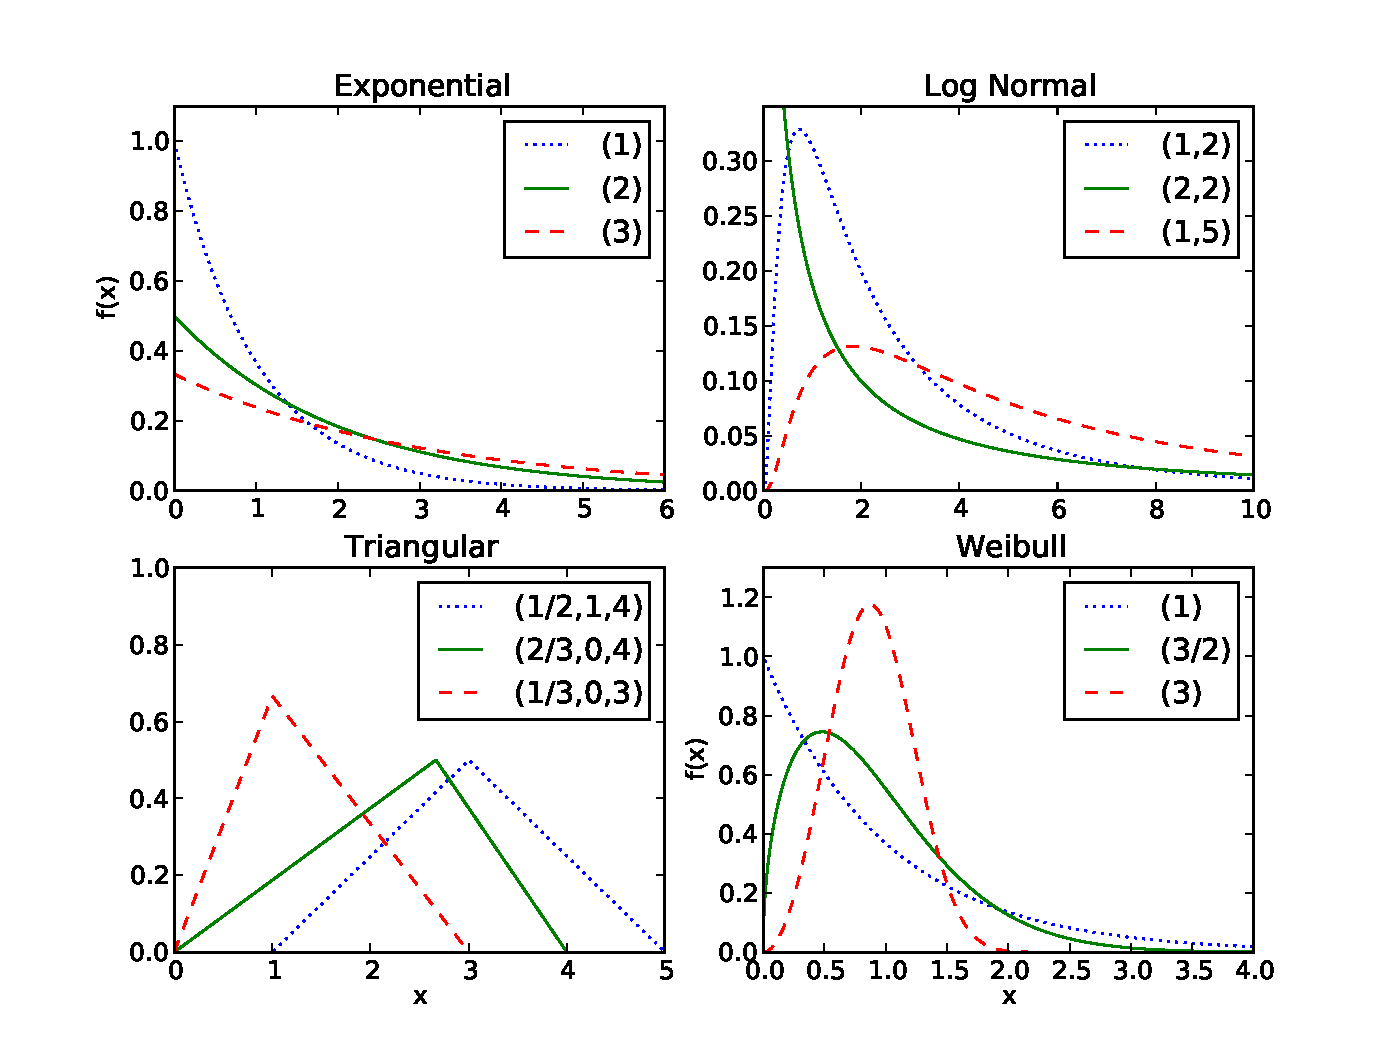
\includegraphics[width=\linewidth]{./graphics/distros_alt}
\caption{Alternate Distributions}
\label{fig:distros_alt}
\end{figure}
\subsection{Exponential}
The exponential distribution ranges from 0 to $\infty$ and has the form
\begin{equation}
\xi(x;\alpha=\alpha e^{-\alpha x}, x\in [0,\infty),
\end{equation}
where $\alpha$ is a rate scaling factor. TODO finish.

\subsubsection{Lognormal}
The log normal is descriptively the log of the normal distribution.  It ranges from 0 to $\infty$ and has the form
\begin{equation}
\xi(x;\mu,\sigma^2)=\frac{1}{x\sqrt{2\pi\sigma^2}}\exp\left(-\frac{(\ln x-\mu)^2}{2\sigma^2}\right),
  \hspace{10pt} x\in(0,\infty).
\end{equation}
where $\mu,\sigma^2$ are the mean and variance, respectively.  TODO finish.

\subsubsection{Triangular}
The triangular distribution ranges from $a$ to $b$ and rises linearly from $a$ to a point, after which it falls linearly to $b$.  The pdf is given by
\begin{equation}
\xi(x;a,b,c)=\begin{cases}
0, & x<a,\\
\frac{2(x-a)}{(b-a)(c-a)}, & a\leq x \leq c,\\
\frac{2(b-x)}{(b-a)(b-c)}, & c<x\leq b,\\
0, & b<x,
\end{cases}
\end{equation}
where $a,b,c$ are the minimum, maximum, and location of the highest point, respectively. TODO finish.

\subsubsection{Weibull}
The Weibull distribution ranges from 0 to $\infty$ and has the form
\begin{equation}
\xi(x;\lambda,k)=\frac{k}{\lambda}\left(\frac{x}{\lambda}\right)^{k-1}e^{-(x/\lambda)^k},
\end{equation}
where $\lambda,k$ are the scale and shape parameters, respectively.  Often, $\lambda=1$ and $k$ is the only shaping parameter. TODO finish.

\subsubsection{Truncated Gaussian}
The truncated Gaussian distribution ranges from $a$ to $b$ and appears as a Gaussian normal distribution truncated at $a$ and $b$ with mean $\mu$ and varianve $\sigma^2$:
\begin{equation}
\xi(x;\mu,\sigma,a,b)=\frac{\frac{1}{\sigma}g(\frac{x-\mu}{\sigma})}{G(\frac{b-\mu}{\sigma})-G(\frac{a-\mu}{\sigma})},
    \hspace{10pt} x\in[a,b],
\end{equation}
where $g$ is the pdf of a normal distribution with $\mu=0,\sigma^2=1$ and $G$ is its cdf.  This can be rewritten as
\begin{equation}
\xi(x;\mu,\sigma,a,b)=\frac{1}{2\sqrt{s\pi\sigma^2}}\left(
\frac{\exp\left(-\frac{(x-\mu)^2}{2\sigma^2}\right)}{\erf(\frac{b-\mu}{\sigma\sqrt{2}})-\erf(\frac{a-\mu}{\sigma\sqrt{2}})}
\right),\hspace{10pt} x\in[a,b],
\end{equation}
where erf is the error function.

\subsubsection{Arbitrary}
Many other distributions may arise in characterizing the uncertainty of input parameters.  In the event none of the above distributions are close enough, using the distribution's ppf to represent it using shifted Legendre polynomials is recommended, with care for the number of terms used.
\end{document}


\begin{center}
\begin{tabular}{c c|c c| c}
\end{tabular}
\end{center}


\begin{figure}[h!]
\centering
\includegraphics[width=\linewidth]{}
\caption
\label{}
\end{figure}